% chktex-file 2
% chktex-file 12
% chktex-file 13

% \documentclass{beamer}
% Without animated slides
\documentclass[handout]{beamer}

% chktex-file 1

\usetheme{Darmstadt}
% More themes at https://www.overleaf.com/learn/latex/Beamer

% --- Packages ---
\usepackage[T1]{fontenc}
\usepackage{lmodern}
\usepackage{amssymb, amsmath}
\usepackage[UKenglish]{datetime}
\usepackage{siunitx} % Writing SI units
\usepackage[most]{tcolorbox}
\usepackage{xcolor}

\newcommand{\mathhighlight}[2]{%
  \tcbhighmath[
    enhanced,
    frame hidden,
    colback=#1,
    boxsep=3pt,
    top=0pt,
    bottom=0pt,
    left=0pt,
    right=0pt,
  ]{#2}
}

\colorlet{highyellow}{yellow!35}
\colorlet{highred}{red!20}
\colorlet{highblue}{cyan!20}
\colorlet{highgreen}{green!20}

\usepackage[
    backend = biber,
    style   = nature,
    isbn    = false
]{biblatex} % BibTeX for bibliography
\usepackage{graphicx, multimedia}

\hypersetup{
    colorlinks=true,
    linkcolor=blue,
    urlcolor=blue,
    citecolor=blue
}

\sisetup{
  per-mode = power
}

% --- Bullet points ---
\setbeamertemplate{itemize item}{\(\bullet\)}
\setbeamertemplate{itemize subitem}{\(\circ\)}
\setbeamercovered{transparent}

% --- Bottom navigation bar ---s
% \setbeamertemplate{navigation symbols}{}
\setbeamertemplate{navigation symbols}{%
    \insertslidenavigationsymbol    % Slide navigation
    \insertframenavigationsymbol    % Frame navigation
    % \insertsubsectionnavigationsymbol    % Subsection navigation
    \insertsectionnavigationsymbol  % Section navigation
    \insertdocnavigationsymbol      % Search / doc navigation
    % \insertbackfindforwardnavigationsymbol % Back/forward arrows

    \usebeamerfont{footline}%
    \usebeamercolor[fg]{footline}%
    \raisebox{1.2pt}[0pt][0pt]{\insertframenumber/\inserttotalframenumber}
}
\setbeamertemplate{sections in toc}[sections numbered]

% --- Custom Commands ---
\newcommand\partialdev[2]{\frac{\partial #1}{\partial #2}}
\newcommand\codev[2]{\frac{D #1}{D #2}}
\renewcommand\d{\mathrm{d}}
\newcommand\dev[2]{\frac{\d #1}{\d #2}}
\newcommand\devsq[2]{\frac{\d^2 {#1}}{\d {#2}^2}}
\addbibresource{bibliography.bib}
\AtBeginBibliography{\scriptsize}

\usepackage{tikzsymbols}

\title{Oceanic Mixed Bottom Layers}
\institute[Department of Applied Mathematics and Theoretical Physics]{
    Department of Applied Mathematics and Theoretical Physics \\
    University of Cambridge
}
\subtitle{Summer Research Festival 2026}
\author{Xing Yu Yi (xyy22), Tian Lang Liu (tll46)}
\date{Monday 12th October 2026}
\titlegraphic{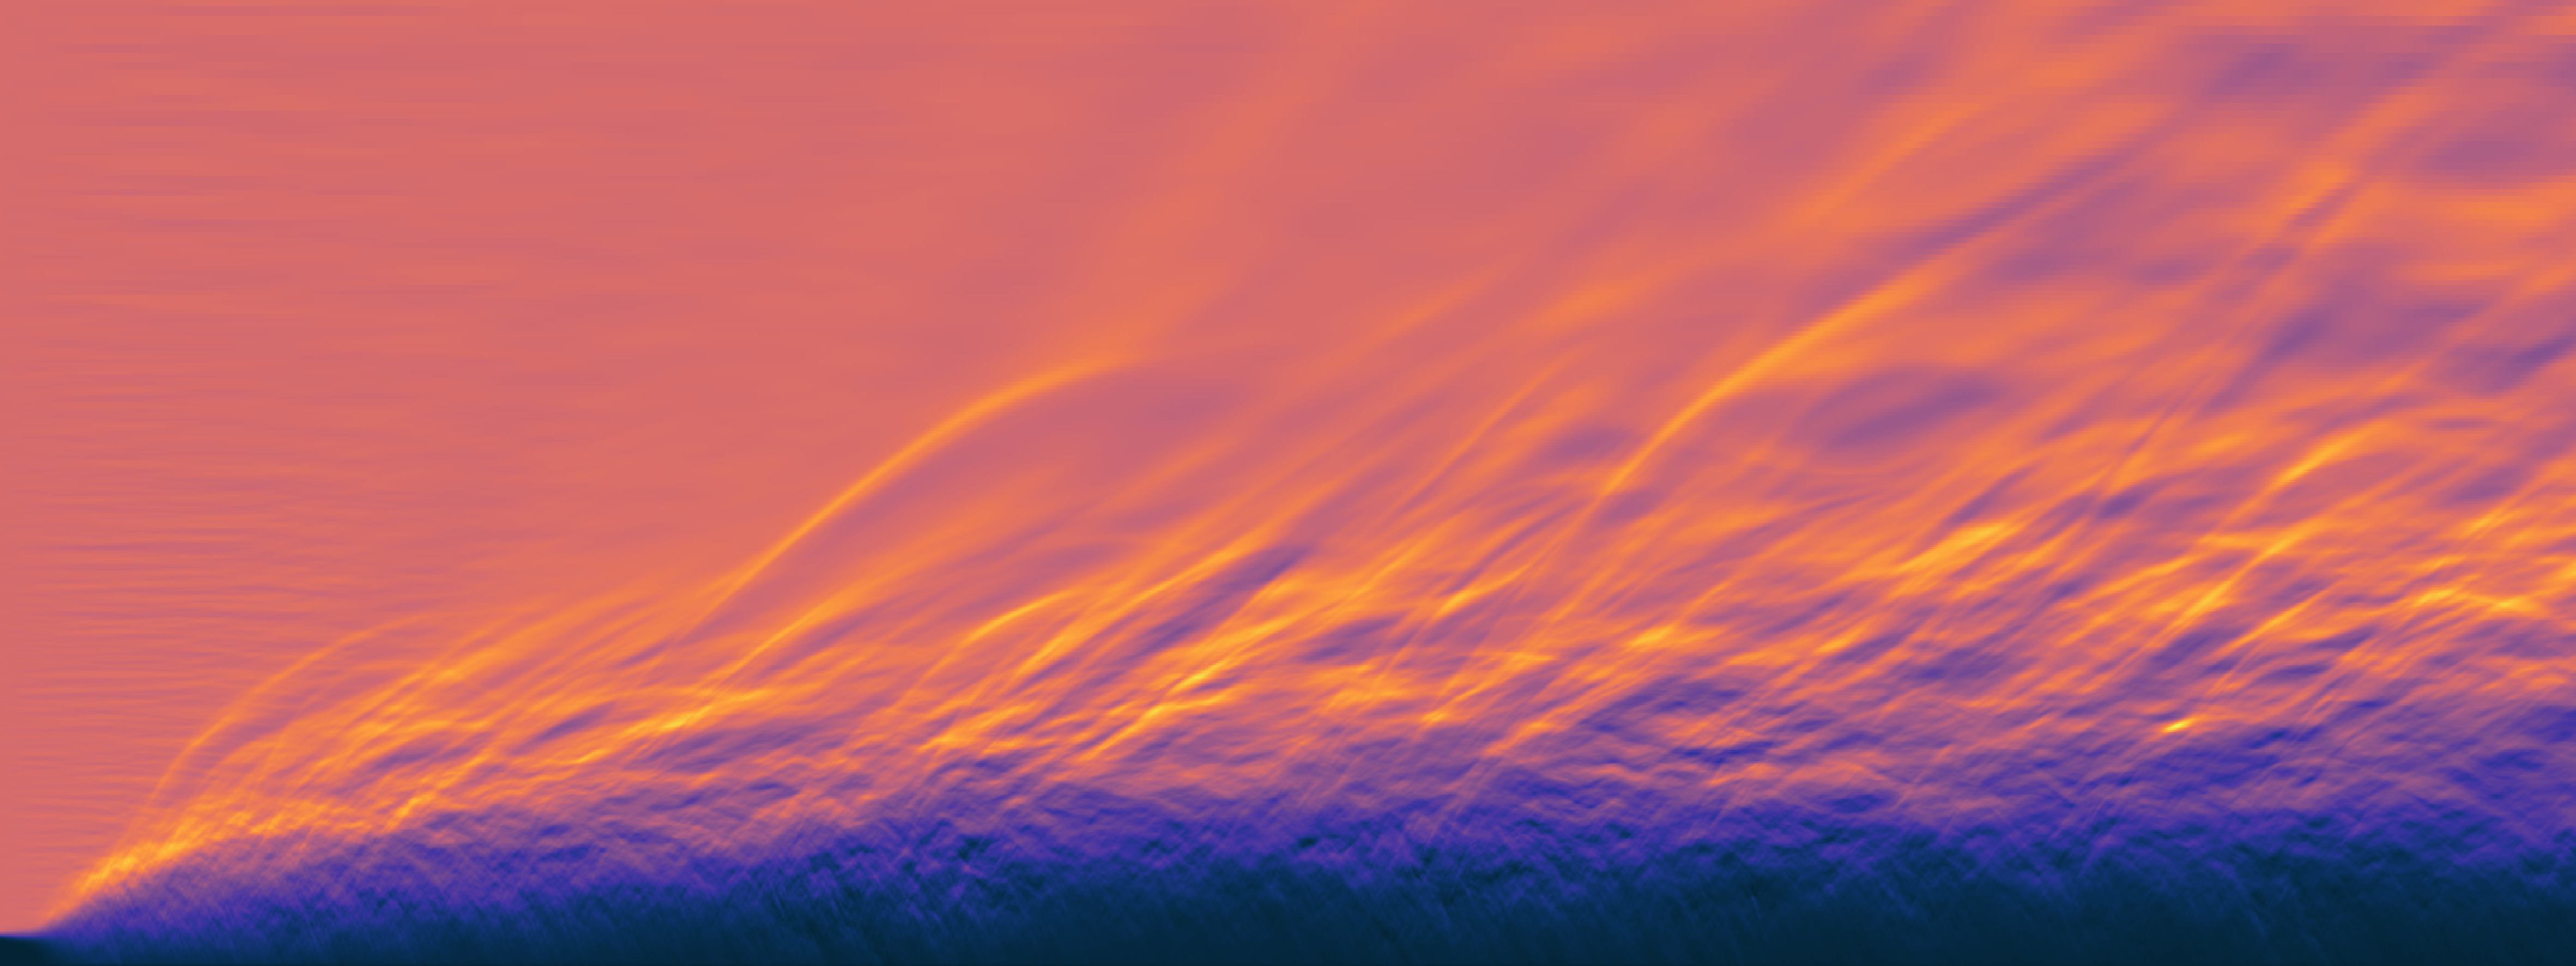
\includegraphics[width=0.45\textwidth]{Figures/Ekman/ekman.png}}

\begin{document}

{
\setbeamertemplate{headline}{}
\maketitle
}

\begin{frame}{Overview}
    \tableofcontents
\end{frame}

% ---------- New section ---------- %
\section{Background}

\begin{frame}{Background}
    Observations in the abyssal ocean show well-mixed layers near the seafloor.

    \begin{itemize}
        \item The Hatteras Abyssal Plain exhibits these bottom mixed layers in the deep ocean. \cite{ArmiMillard76}
        \item Global surveys show especially thick bottom mixed layers in weakly stratified regions. \cite{Huang2019}
        \item The observed layer depth scale with mean current speed, and are affected by background stratification.
    \end{itemize}

    In this project, we explore the following question
    \begin{quote}
        What physical mechanism produces these thick bottom mixed layer (BML)?
    \end{quote}
\end{frame}

\begin{frame}{Hatteras Abyssal Plain}
    \begin{figure}[!htbp]
    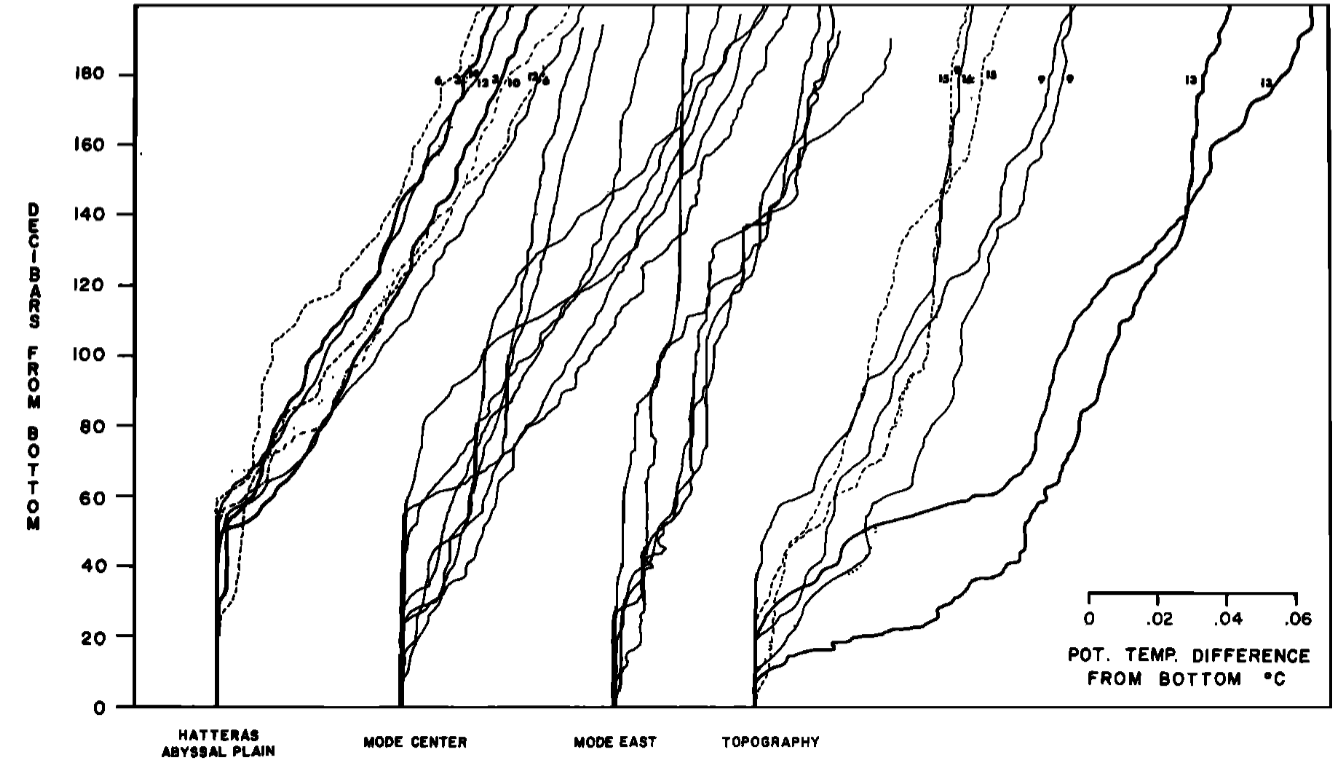
\includegraphics[width=0.75\textwidth]{Figures/Ekman/hatteras.png}
    \caption{Potential temperature profiles relative to ocean bottom at various locations around Hatteras Abyssal Plain. \cite{ArmiMillard76}}
    \end{figure}
\end{frame}

\begin{frame}{Causes of thick BML}
    As we have a mixing process to generate turbulence, we investigate potential sources of energy:
    \begin{itemize}[<+->]
        \item \emph{Benthic storms}: episodic bursts of intense bottom currents, with typical speeds \(\sim\)\,\qty{20}{\centi\metre\per\second} over weeks
        \item \emph{Tides}: periodic barotropic tidal current with typical speeds on the order of \qtyrange{1}{2}{\centi\metre\per\second}, more important near sloped topographies
        \item \emph{Wave breaking}: internal wave breaking inducing turbulence
    \end{itemize}
\end{frame}

\begin{frame}{Approximations}
    \begin{itemize}[<+->]
        \item \emph{Boussinesq approximation}: negligible density variations \(\rho' \ll \rho_0\), with only momentum contribution to buoyancy
        \item \emph{Incompressibility}: assume we have incompressible flow \[\nabla\cdot\mathbf{u} = 0\]
        \item \emph{Mass conservation/continuity equation}:
        \[\partialdev{\rho}{t} + \nabla\cdot(\rho\mathbf{u}) = 0 \quad \iff \quad \codev{\rho}{t} = 0\]
    \end{itemize}
\end{frame}

% ---------- New section ---------- %
\section{Ekman model}

\begin{frame}{Classical Ekman layer near rigid boundary}
    Assume far-stream flow  \(U_\infty \hat{\mathbf{x}}\) in geostrophic balance far from rigid boundary at \(z=0\):
    \[fU_\infty = -\frac{1}{\rho}\partialdev{p}{y}\]
    Also, assume vertical flow lengthscale \(\ll\) ``scale height'' of medium \(\sim c^2/g\).

    Ekman layers form due to balance of \emph{Coriolis} and \emph{friction} forces.
\end{frame}

\begin{frame}{Analytic solution for Ekman layer}
    With \(f\)-plane approximation, where  Coriolis parameter \(f=2\Omega\sin\theta\), look for steady-state solution:
    \[
        -fv = \nu \devsq{u}{z}\,, \quad
        fu = \nu \devsq{v}{z} + fU_\infty.
    \]
    \emph{Boundary conditions:} \(u=v=0\) at \(z=0\), and \((u,v) \to (U_\infty, 0)\) as \(z \to \infty\).

    Rewrite \(V=u+iv\), analytic solution
    \[V = U_\infty\left[1-\exp\left(-\frac{(1+i)z}{\delta_E}\right)\right]\,\]
    where \(\delta_E = \sqrt{2\nu/f}\).
\end{frame}

\begin{frame}{Analytic solution for Ekman layer}
    \begin{figure}[htbp]
        \centering
        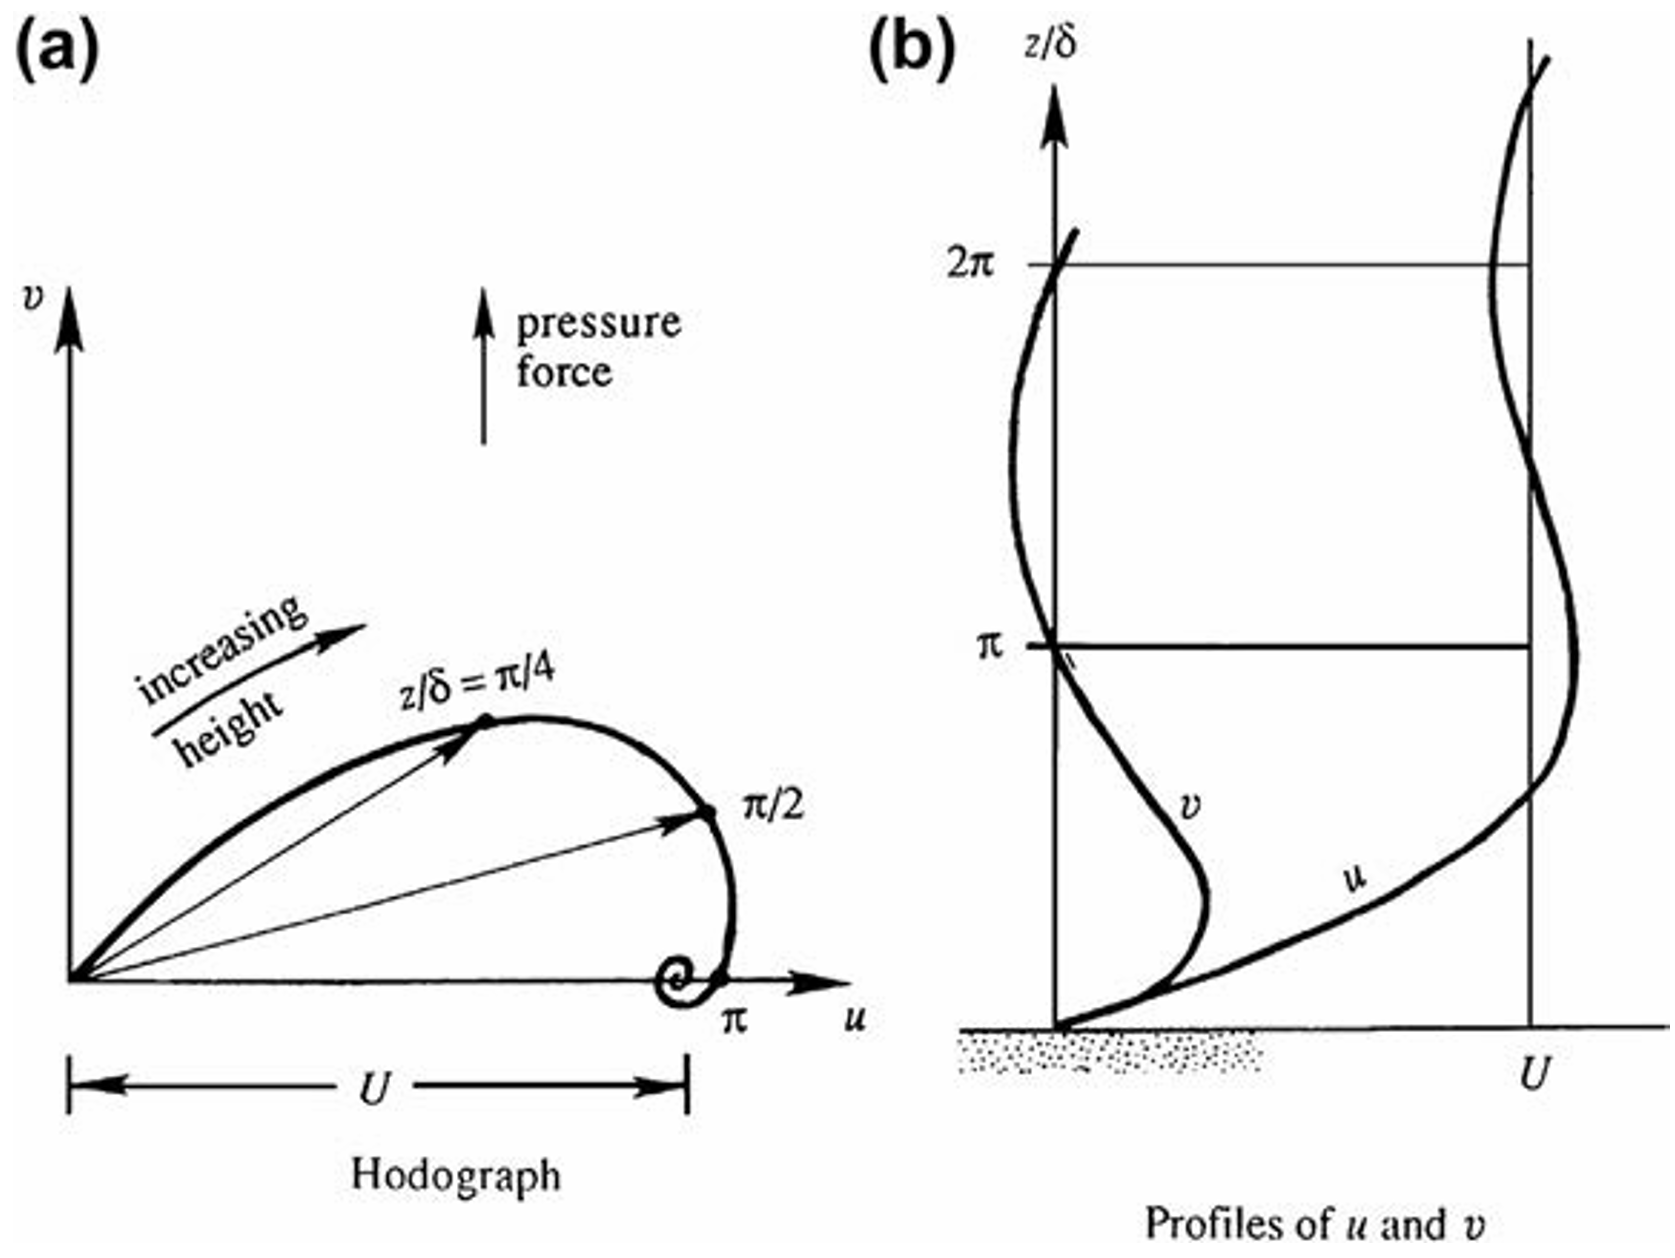
\includegraphics[height=0.6\textheight]{Figures/Ekman/spiral.png}
        \caption{Plot of analytic solution for Ekman layer at rigid boundary on a hodograph, and velocity components with depth. \cite{Kundu2015}}
    \end{figure}
\end{frame}

\begin{frame}{Setup for Ekman model}
    \begin{align}
    \codev{u}{t} - fv &= -\partialdev{p}{x} + \partialdev{\tau_{xz}}{z} \\
    \codev{v}{t} + fu &= -\partialdev{p}{y} + \partialdev{\tau_{yz}}{z} \mathhighlight{highblue}{+ fU_\infty}
    \end{align}
    \begin{itemize}
        \item Far-stream velocity \(U_\infty \hat{\mathbf{x}}\)
    \end{itemize}
\end{frame}

% ---------- New section ---------- %
\section{Stokes model}

\begin{frame}{Setup for Stokes model}
    \begin{align}
    \codev{u}{t} &= -\partialdev{p}{x} + \partialdev{\tau_{xz}}{z} + \mathhighlight{highblue}{U_0 \omega \cos \omega t} \\
    \codev{v}{t} &= -\partialdev{p}{y} + \partialdev{\tau_{yz}}{z}
    \end{align}

    \begin{itemize}[<+->]
        \item Far-stream oscillatory velocity \(U_0 \hat{\mathbf{x}}\sin \omega t\)
        \item No Coriolis effects
    \end{itemize}
\end{frame}

% ---------- New section ---------- %
\section{Simulating the BML}

\begin{frame}{Simulating both models}
    \begin{itemize}
        \item Simulate bottom mixed layer (BML) evolution for both Ekman and Stokes models
        \item Use \emph{Oceananigans.jl} in Julia for simulations
        \item Domains: vertical extent \(\sim\) \qty{100}{\metre}, time evolution \(\sim\) 10 days
    \end{itemize}
\end{frame}

\begin{frame}{Animation}
    \begin{figure}
        \centering
        \movie[externalviewer]{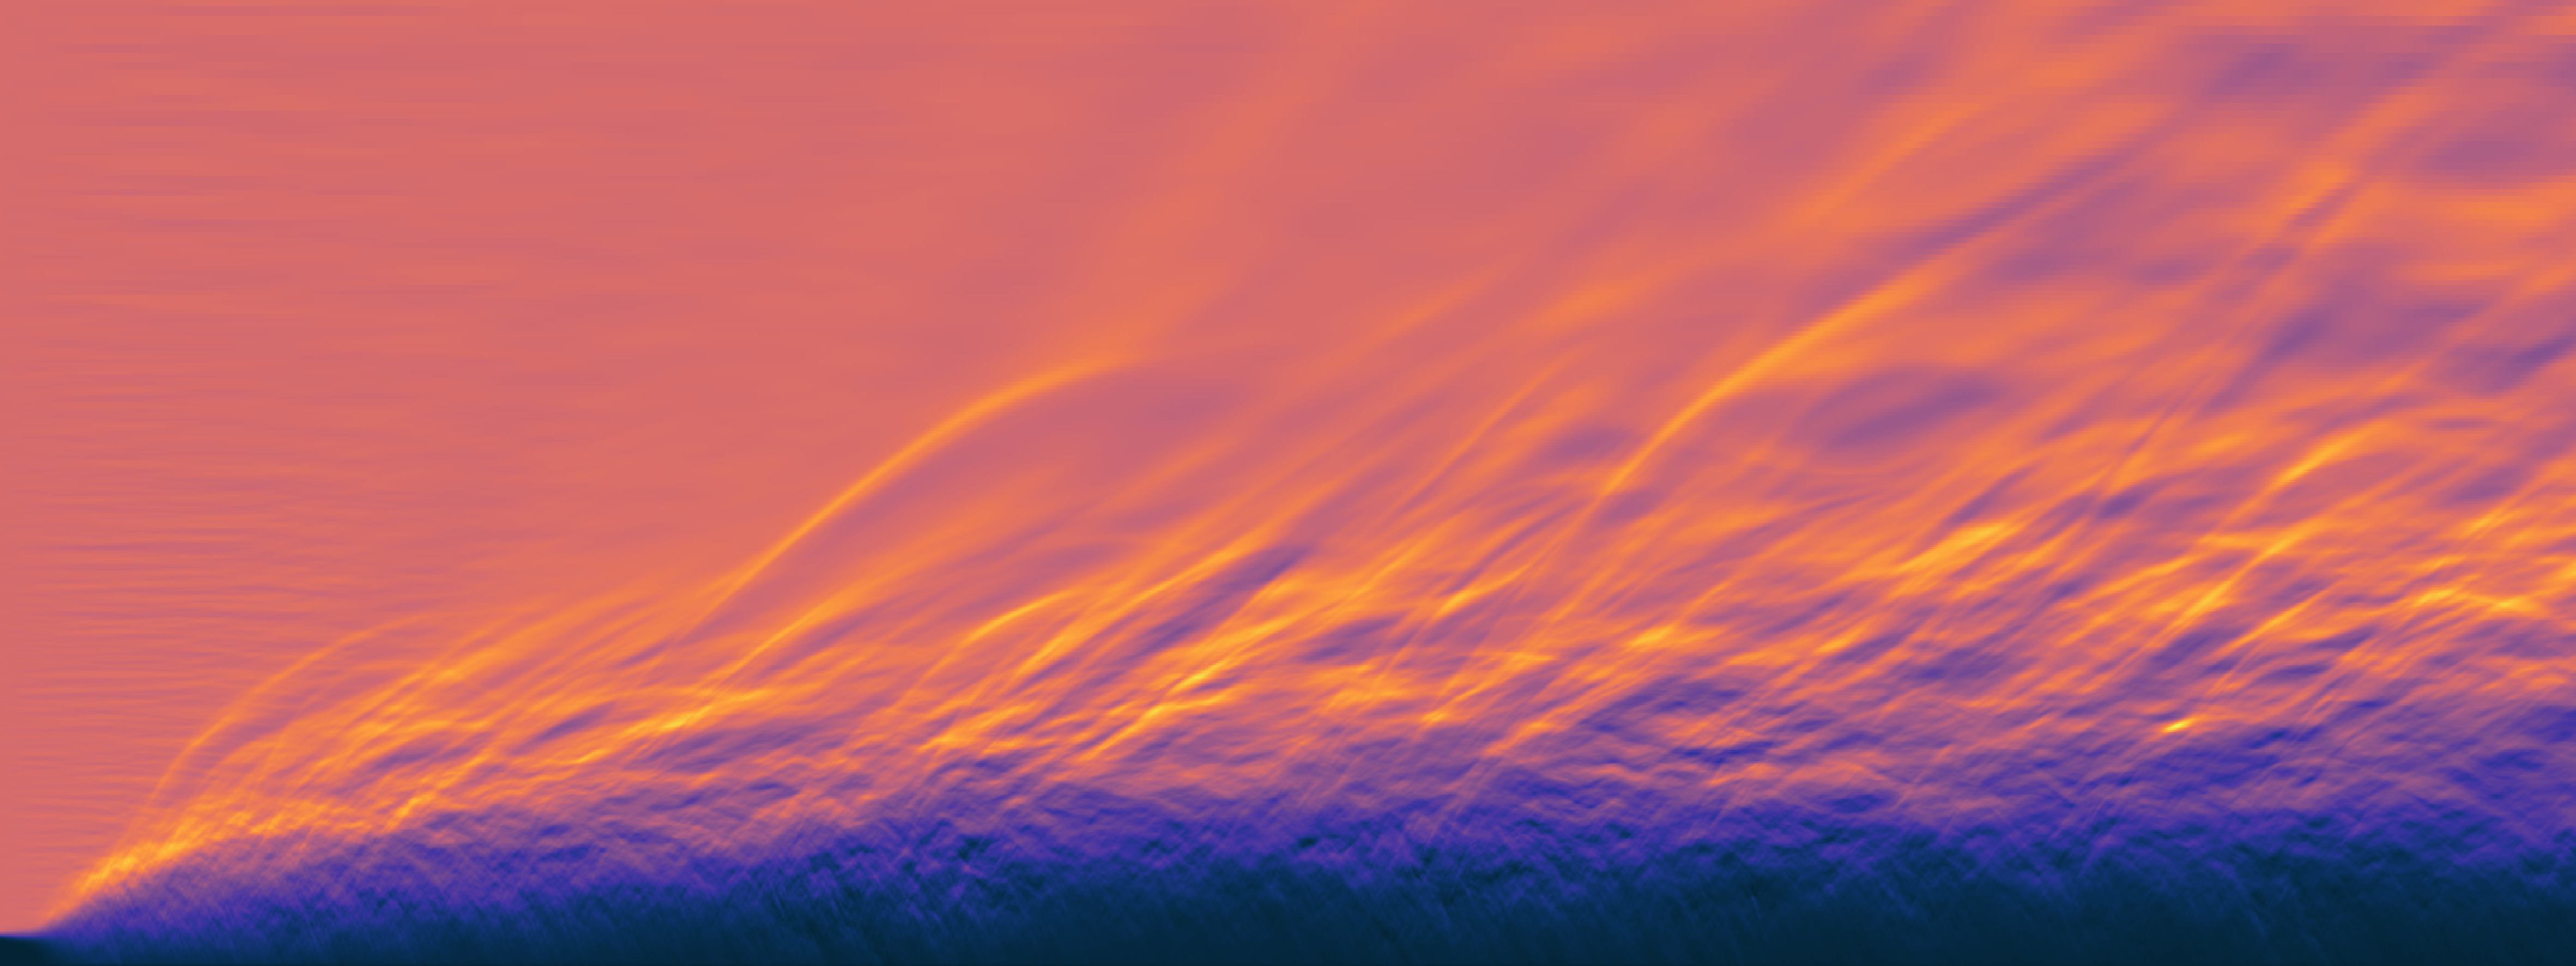
\includegraphics[width=0.75\textwidth]{Figures/Ekman/ekman.png}}{Figures/Ekman/r=0.mp4}
        \caption{Ekman flow animation}
    \end{figure}
\end{frame}

\begin{frame}{Key simulation parameters}
    \begin{itemize}[<+->]
        \item \emph{Initial stratification}: uniform density with thin interface above bed
        \item \emph{Far-stream current}: $U_\infty = \qty{0.1}{\metre\per\second}$ (typical abyssal)
        \item \emph{Stokes drift amplitude}: $U_s(0) = 0.02 U_\infty$ at bed (wave contribution)
        \item \emph{Grid}: high resolution near bottom (\(\sim\)\qty{0.5}{\metre}), coarser above
        \item \emph{Monitoring}: vertical profiles of buoyancy frequency, velocity, and mixed layer depth
    \end{itemize}
\end{frame}

% ---------- New section ---------- %
\section{Predicting BML evolution}

\begin{frame}{Comparing both models}
    Here's some maths
\end{frame}

% ---------- New section ---------- %
\section{Summary}

\begin{frame}{Summary}
    \begin{itemize}
        \item
    \end{itemize}
\end{frame}

\begin{frame}{Thank you!}
    Many thanks to our supervisors Prof. John Taylor, Dr Bethan Wynne-Cattanach, and Dr Yuchen Ma, and all the other wonderful people we have been grateful to meet on SRIM! \Laughey{} \vspace{1ex}

    \begin{center}
        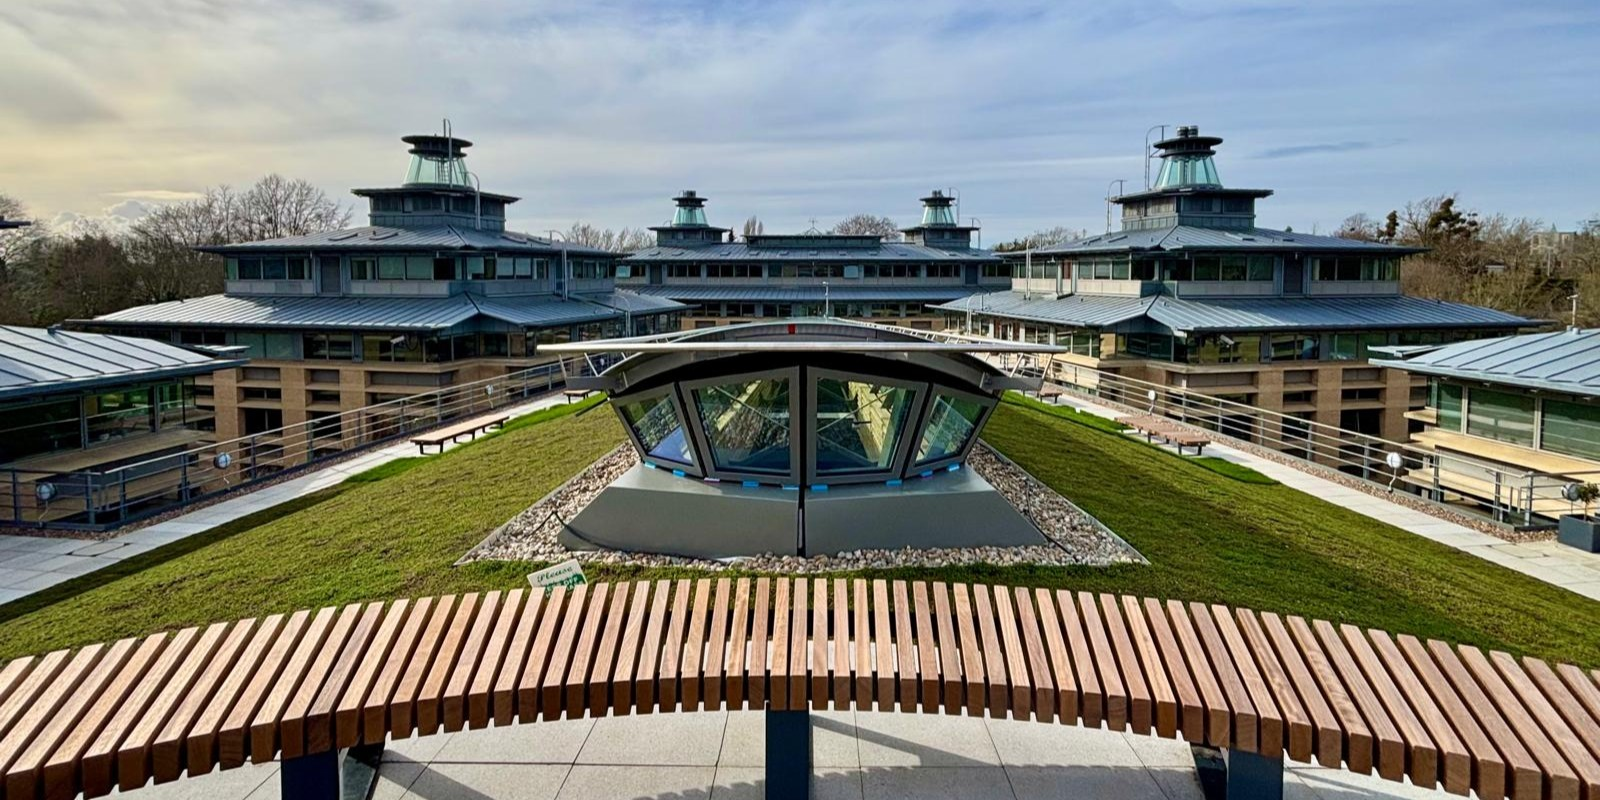
\includegraphics[width=0.6\textwidth]{Figures/cmsrooftop.jpg}
    \end{center}
\end{frame}

\begin{frame}{References}
    \nocite{TaylorSarkar2008}
    \nocite{WeatherlyMartin78}
    \printbibliography
\end{frame}

\end{document}